\documentclass[a4paper, 14pt]{extarticle}

\usepackage[utf8]{inputenc}

% Подключение и настройка внешнего вида гиперссылок
\usepackage{xcolor}
\usepackage[unicode]{hyperref}
\definecolor{LINKCOLOUR}{rgb}{0.1,0.0,0.9}
\hypersetup{colorlinks,breaklinks,urlcolor=LINKCOLOUR,linkcolor=LINKCOLOUR}

% Выбор внутренней TEX−кодировки
\usepackage[T2A]{fontenc}

% Включение переносов для русского и английского языков
\usepackage[english,russian]{babel}

\usepackage{hyphenat}
\selectlanguage{english}
\hyphenation{
    MAT-LAB Si-mu-link
    Tel-co Mo-ti-on
    Tex-as Inst-rum-ents
}
\selectlanguage{russian}
\hyphenation{
    уп-рав-ле-ни-е уп-рав-ле-ни-я уп-рав-ле-ни-ем уп-рав-ле-ний
    нес-коль-ко
    об-ос-но-ва-ни-е об-ос-но-ва-ни-я об-ос-но-ва-ни-ий об-ос-но-ва-ни-ем
}

% Начинать первый параграф раздела следует с красной строки
\usepackage{indentfirst}

\usepackage{caption}
\captionsetup[figure]{labelfont=bf, justification=centering}
\captionsetup[table]{labelfont=bf, justification=centering}

%\usepackage{weird,querr}
\usepackage{amssymb}
\usepackage{amsmath}

\usepackage{cmap}

\usepackage{longtable}
\usepackage{multirow}

\usepackage{tabu}
\tabulinesep=1mm    % минимальное расстояние между содержимым ячейки tabu
                    % и границей ячейки

\usepackage{geometry}   % Меняем поля страницы
\geometry{left=2cm}     % левое поле
\geometry{right=1.5cm}  % правое поле
\geometry{top=1.5cm}    % верхнее поле
\geometry{bottom=2.4cm} % нижнее поле

% подавить предупреждение о некорректной версии .pdf
\pdfminorversion=6
% работа с импортом изображений
\usepackage{graphicx}

% Схемы
\usepackage{tikz}
\usetikzlibrary{arrows,calc}
\usepackage{pgfplots}
\pgfplotsset{
  compat=newest,
  xlabel near ticks,
  ylabel near ticks
}

% для вставок листинга кода
% см. http://en.wikibooks.org/wiki/LaTeX/Source_Code_Listings
\usepackage{listings}

\usepackage{pdfpages}

\usepackage{subfiles}

% символ градуса и т.д.
\usepackage{gensymb}

% стилевой пакет, открывающий доступ к большому числу типографских значков
\usepackage{textcomp}

% условие для вставки некоторых частей, присущих диплому, но не нужных в более
% старых документах
\newcommand{\DIPLOMA}

\newcommand\abs[1]{\left|#1\right|}

\newcommand\invisiblesubsection[1]{%
    \refstepcounter{subsection}%
    \addcontentsline{toc}{subsection}{\protect\numberline{\thesubsection}#1}%
    \subsectionmark{#1}%
}

% пустой заголовок при использовании \listoffigures
\addto\captionsrussian{%
    \renewcommand\listfigurename{}%
}

% пустой заголовок при использовании \listoftables
\addto\captionsrussian{%
    \renewcommand\listtablename{}%
}

% пустой заголовок при использовании \bibliography
\addto\captionsrussian{%
    \renewcommand\refname{}%
}

\lstset{
    language=C,
    basicstyle=\small\ttfamily,
    title=\lstname,
    numbers=left,
    breaklines=true,
    breakatwhitespace=false,
    postbreak=\raisebox{0ex}[0ex][0ex]{\ensuremath{\color{red}\hookrightarrow\space}},
    frame=l,
    keywordstyle=\color{teal}
}

\lstset{
    morekeywords={  uint_fast8_t, int_fast8_t, uint_fast16_t, int_fast16_t, uint_fast32_t, int_fast32_t,
                    uint8_t, int8_t, uint16_t, int16_t, uint32_t, int32_t, uint64_t, int64_t, void
                }
}

\begin{document}
% установить значение счетчика страниц, для нумерации не с 1
\setcounter{page}{5}

\tableofcontents

\newpage

\subfile{src/product_requirements.tex}
\newpage
Задачи работы:
\begin{enumerate}
    \item Выбор двигателя, энергетический расчёт
    \item Анализ существующих алгоритмов управления шаговым двигателем
    \item Построение математической модели привода
    \item Синтез алгоритмов управления
    \item Реализация алгоритмов управления
    \item Разработка платы управления
    \item Разработка и изготовление макетного стенда для натурного моделирования
    \item Экспериментальная проверка алгоритмов управления
    \item Разработка технологий сборки платы управления
    \item Разработка технологии макетного стенда
    \item Технико~-- экономическое обоснование выбора основных компонентов
        привода с использованием функцианально~-- стоимостного анализа
    \item Анализ опасных и вредных факторов при разработке и расчёт освещённости
        как наиболее опасного фактора
    \item Анализ влияния техпроцесса изготовления печатной платы и расчёт системы
        вентиляции производственного помещения
\end{enumerate}

\subfile{src/research/all_research.tex}
\subfile{src/construction/all_construction.tex}
\subfile{src/experiments/all_experiments.tex}
\subfile{src/technology/all_technology.tex}
\subfile{src/economics/economics.tex}
\subfile{src/ecology/all_ecology_except_normatives.tex}
\subfile{src/bibliography.tex}

\clearpage
\section{Приложение}
\subsection{Список иллюстраций}
\listoffigures
\clearpage
\subsection{Список таблиц}
\listoftables

\subfile{src/code_listings_include.tex}

\newpage
\invisiblesubsection{Перечень элементов платы управления}
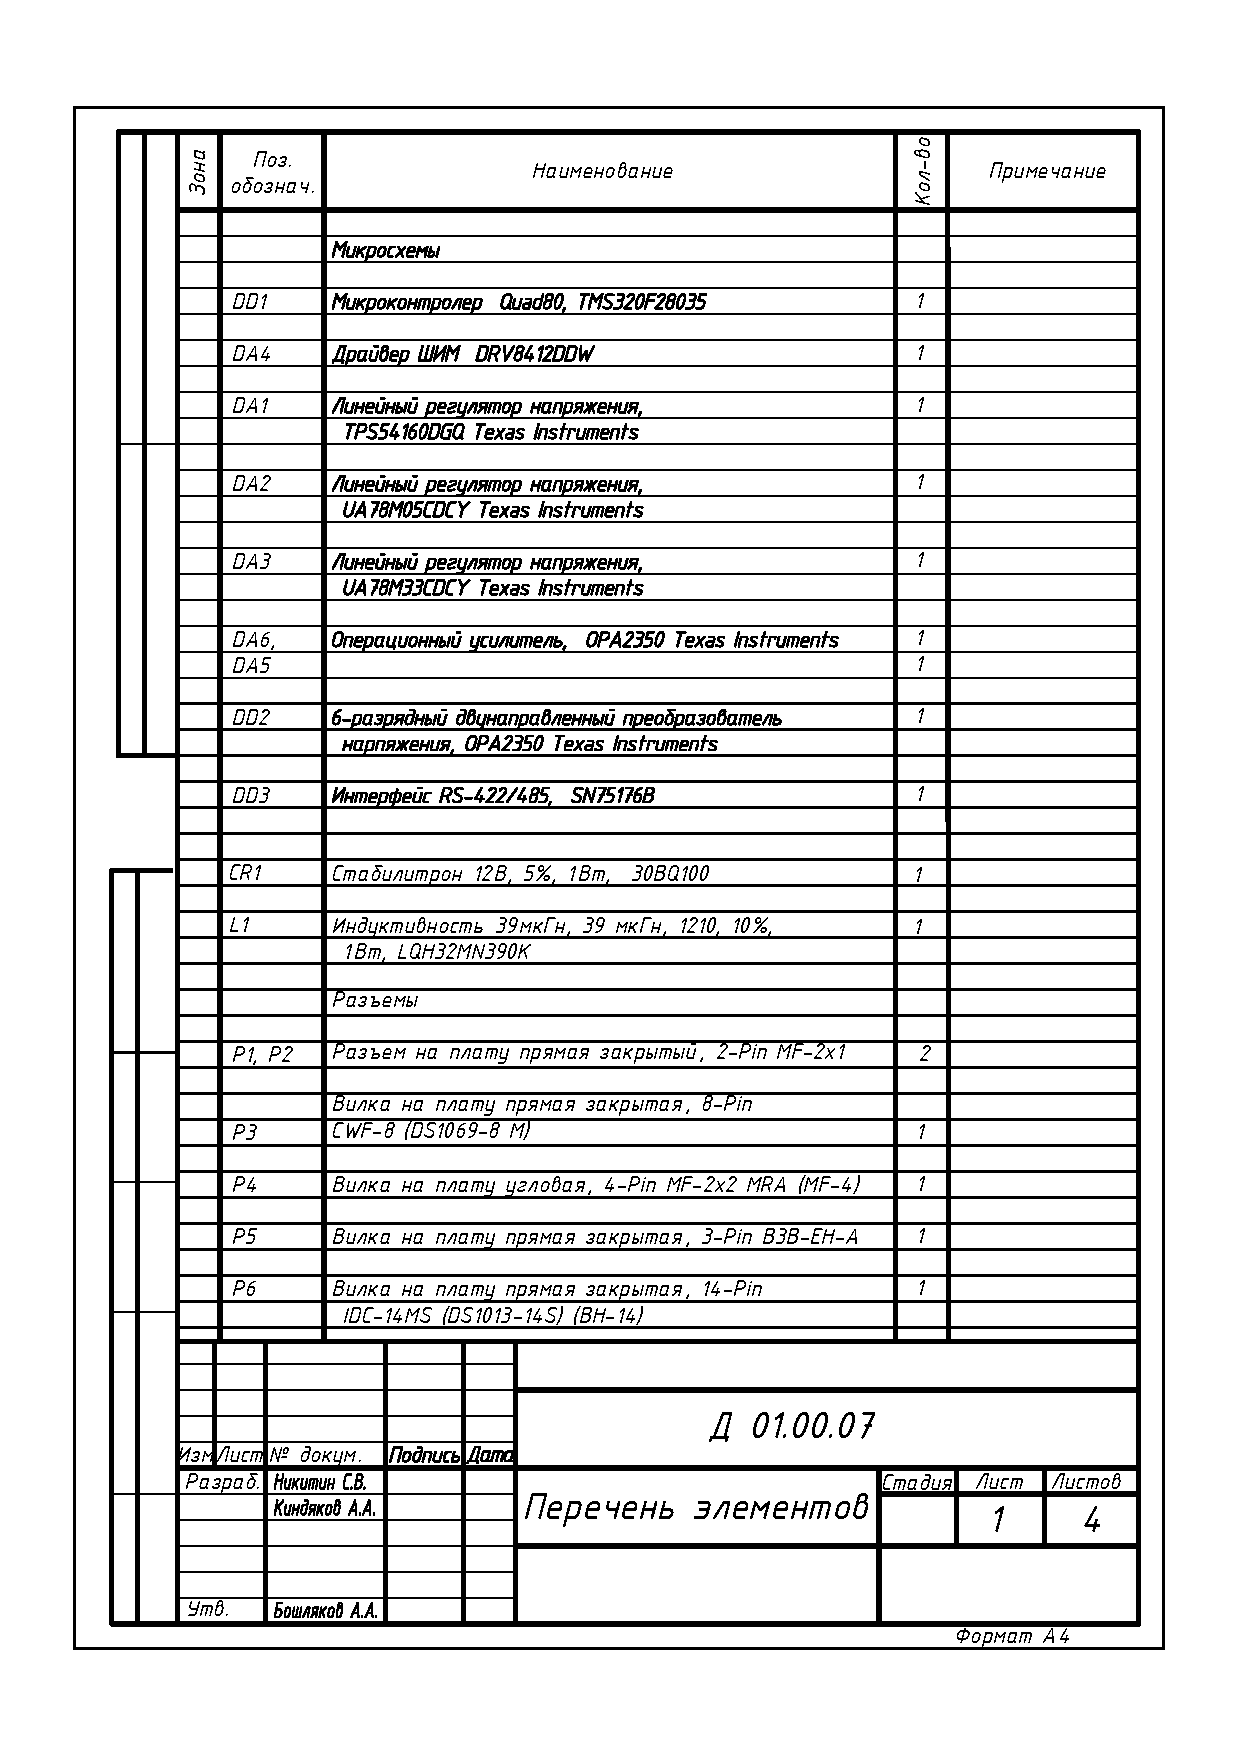
\includepdf[pages=-]{./additional/pcb_bom_list}

\newpage
\invisiblesubsection{Операционные карты техпроцесса сборки платы управления}
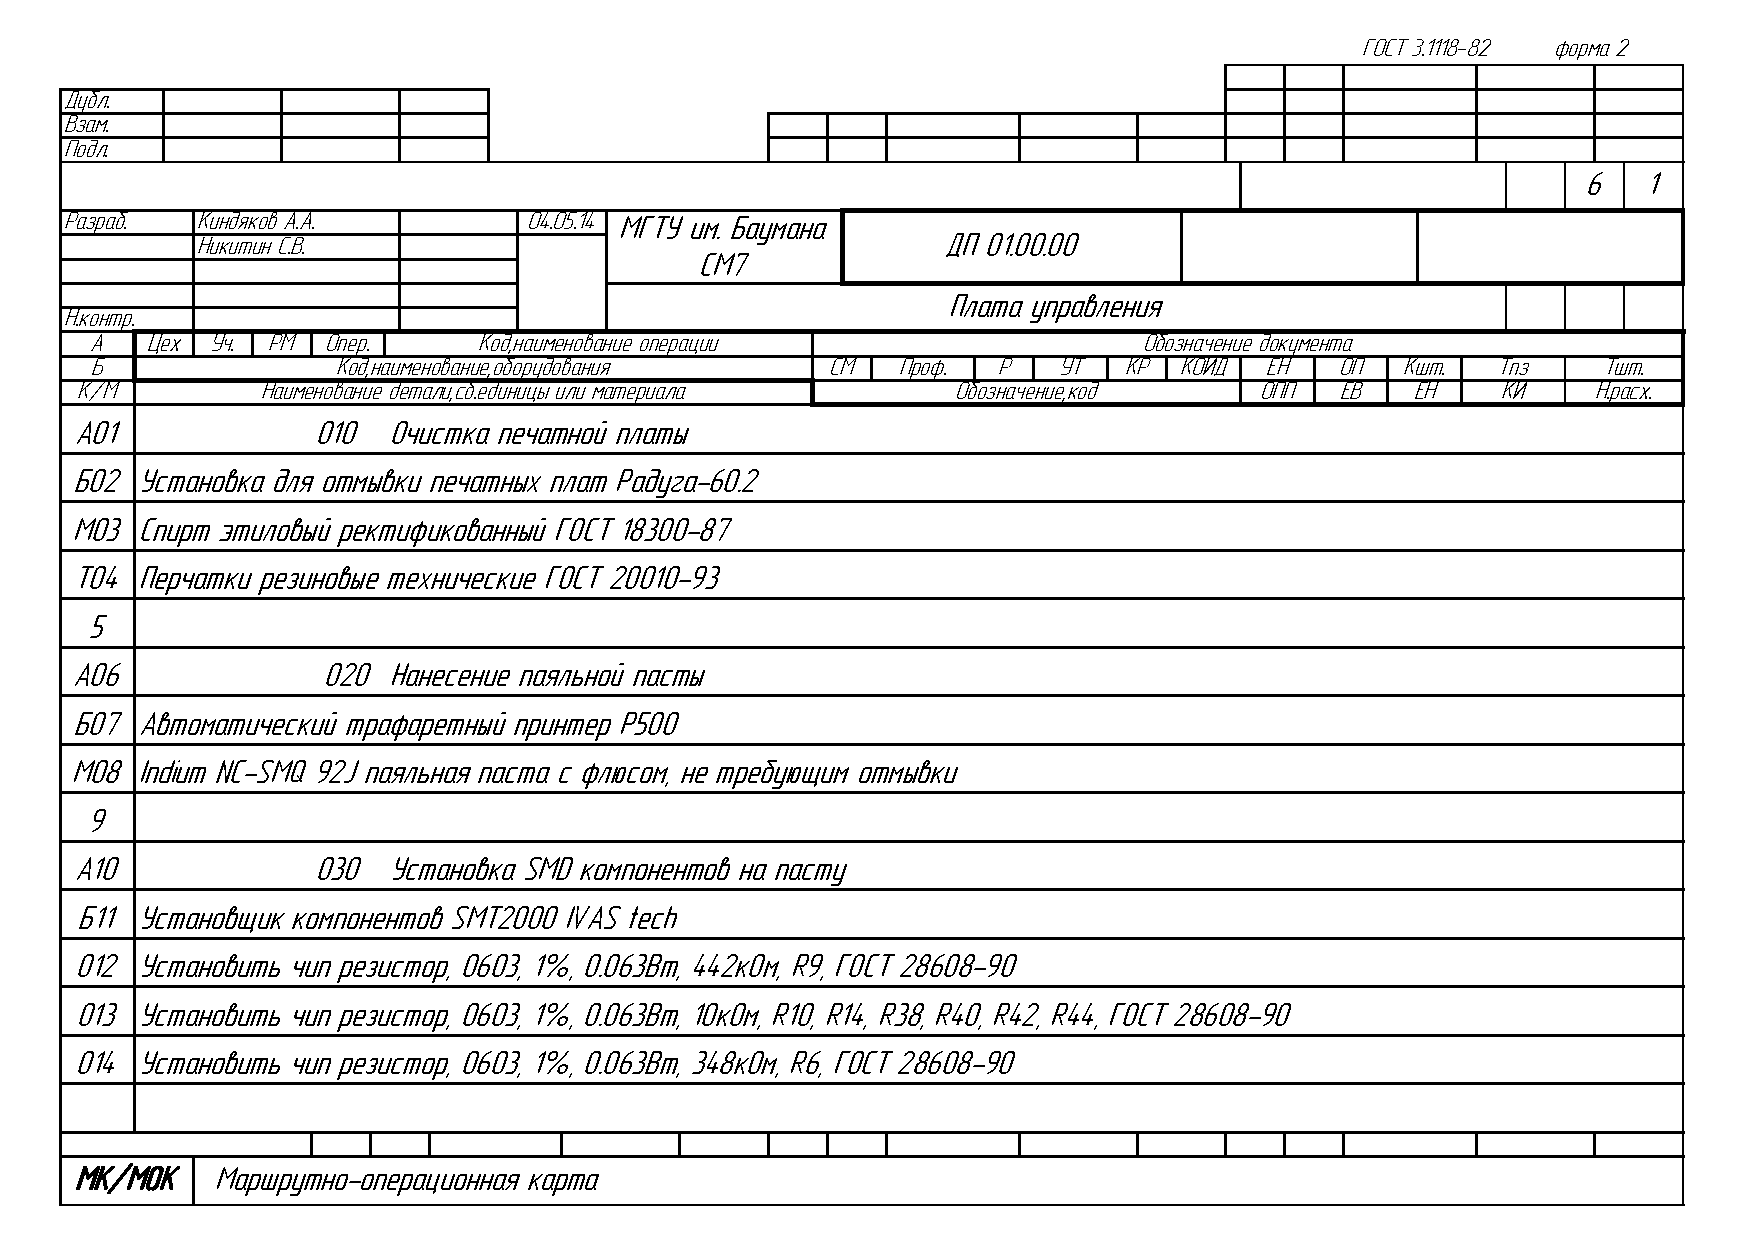
\includepdf[pages=-, angle=90]{./additional/pcb_operational_maps}

\newpage
\invisiblesubsection{Спецификая макетного стенда}
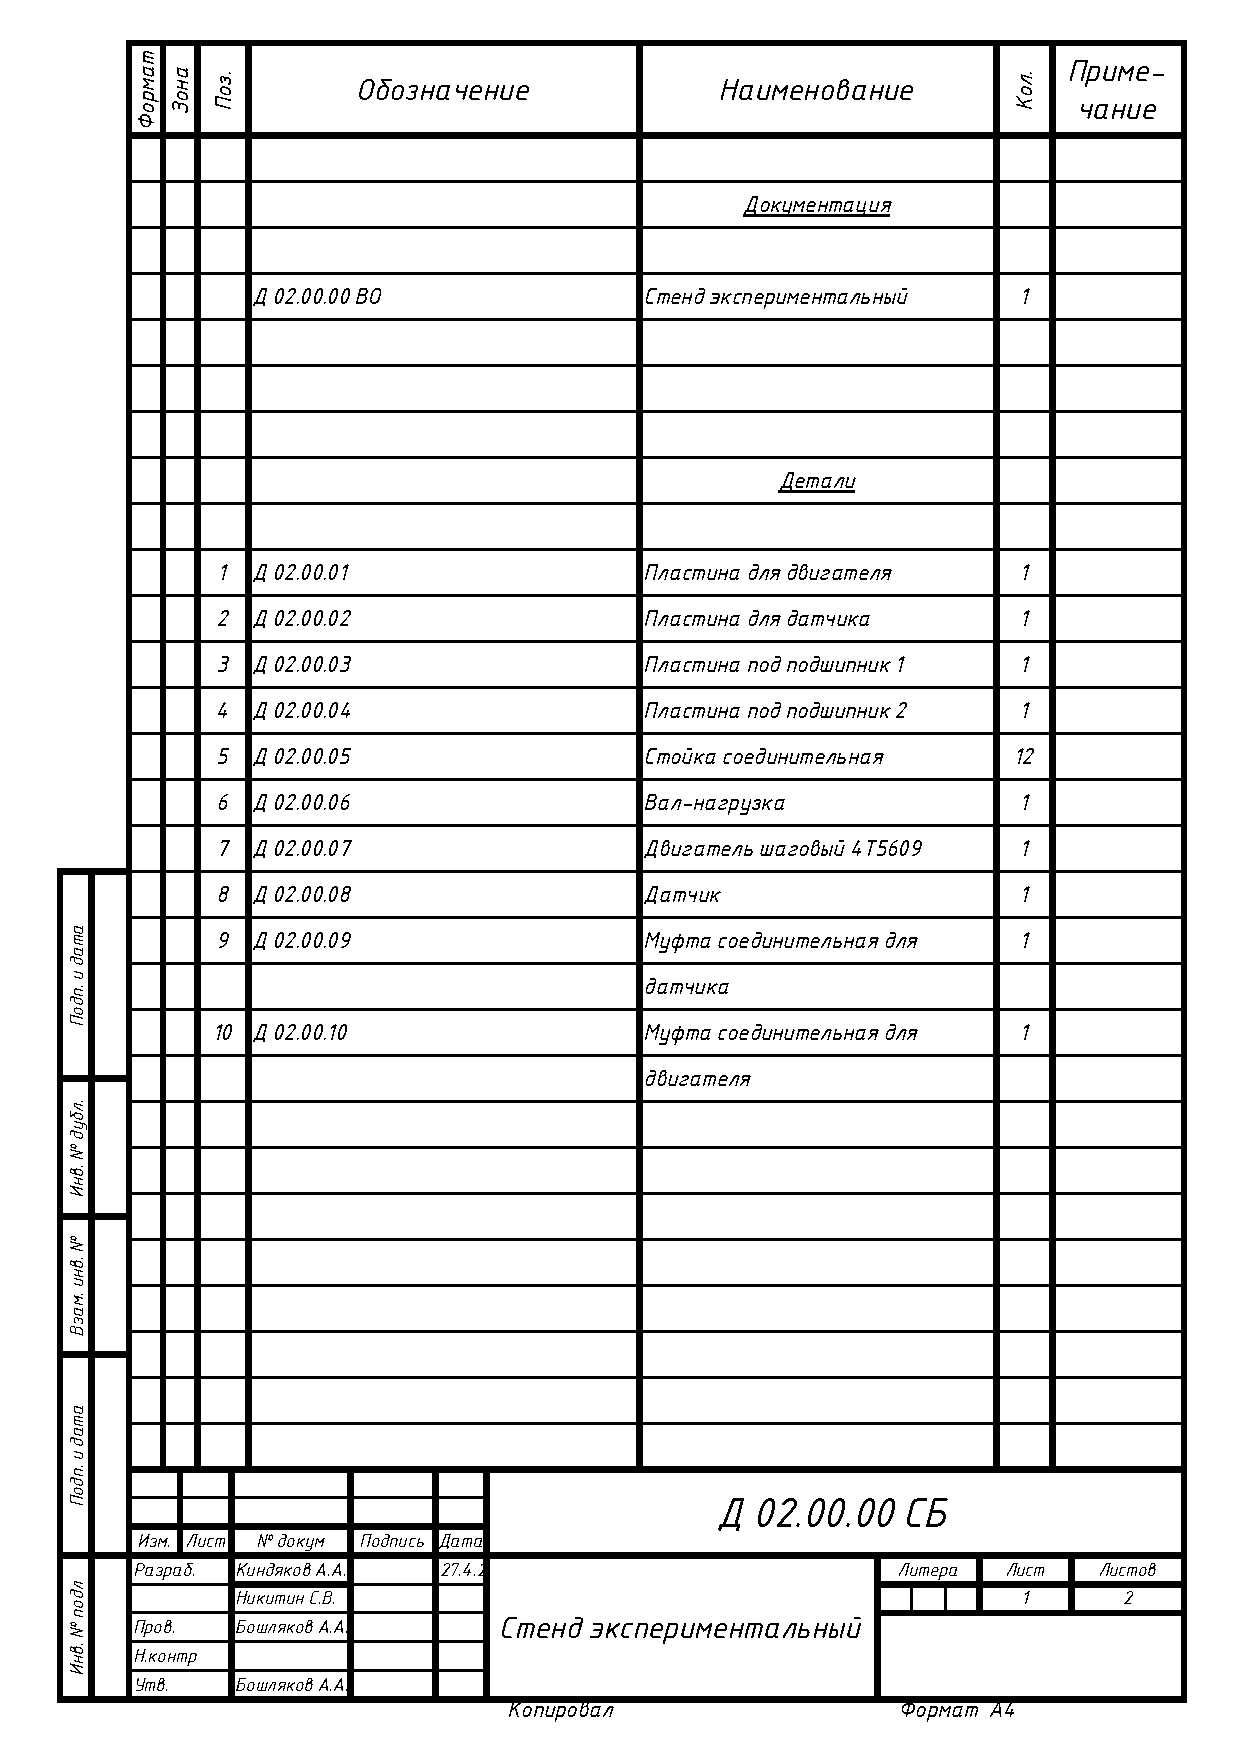
\includepdf[pages=-]{./additional/complete_assembly_spec}

\newpage
\invisiblesubsection{Операционные карты техпроцесса сборки макетного стенда}
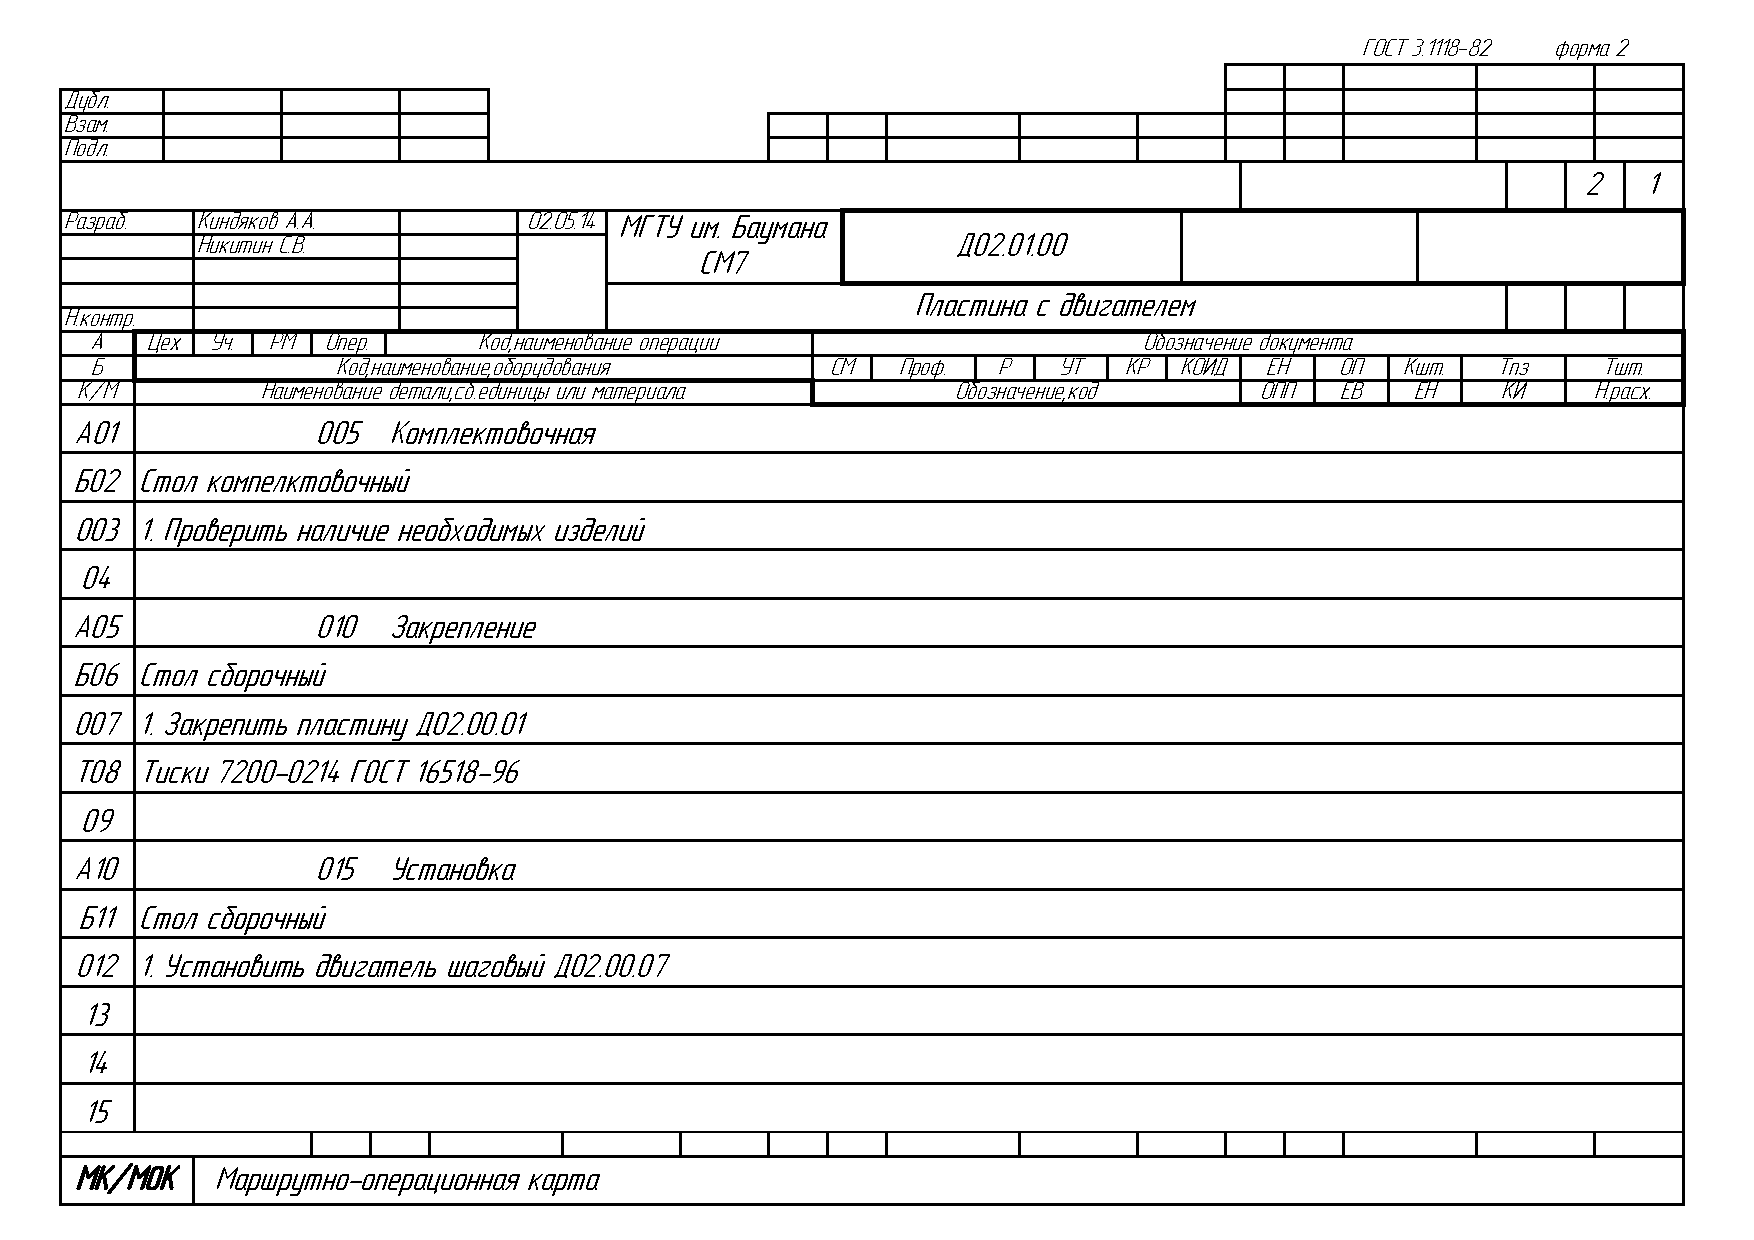
\includepdf[pages=-, angle=90]{./additional/all_operational_maps}

\end{document}
